% В этом файле следует писать текст работы, разбивая его на
% разделы (section), подразделы (subsection) и, если нужно,
% главы (chapter).

% Предварительно следует указать необходимую информацию
% в файле SETUP.tex

\input{preamble.tex}


\NewBibliographyString{langjapanese}
\NewBibliographyString{fromjapanese}

\begin{document}

%\Introduction

%Результаты, полученные в современной математике, становятся всё сложнее. Постепенно подступает момент, когда математики, работающие в разных областях, окончательно перестанут понимать друг друга, а их результаты станет невозможно проверить. Одним из наиболее активно использующихся решений является проверка математических результатов с помощью средств доказательства теорем. Этот класс инструментов сам по себе заслуживает особого внимания, так как было создано множество непохожих подходов, в основе которых лежат интересные теории.
%
%Гомотопическая теория типов (Homotopy type theory, HoTT) \autocite{hottbook} --- относительно новая область в информатике, которая базируется на неожиданной связи между теорией типов и теорией гомотопий. Эта область лежит в основе \textit{Унивалентных оснований математики} (Univalent Foundation, UF) \autocite{UFP2010} --- попытки формализовать математику, используя в качестве основы не множества, а гомотопические типы или $\infty$-группоиды, а также \textit{высшие индуктивные типы} (Higher Inductive Types, HIT). Этот подход в первую очередь интересен тем, что позволяет работать с гомотопической теорией, используя \textit{синтетический метод}, то есть не опираясь на более базовые примитивы, как, например, множества, также очень важным преимуществом HoTT являются хорошие вычислительные свойства, унаследованные от зависимой теории типов Мартин-Лёфа \autocite{MLTT}. Первоначальная версия гомотопической теории типов включала в себя \textit{аксиому унивалентности}, что открыло возможность для формализации крупного пласта математики на теоретико-типовом языке: экстенсиональности функций и равенства структур, между которыми доказано существование изоморфизма. Но у этой версии было одно очень важное ограничение --- аксиома не имела вычислительной интерпретации. В данный момент наиболее многообещающим решением является использование \textit{кубической теории типов} \autocite{CohenCHM16}, в которой эта аксиома является теоремой, имеющей конструктивное доказательство.
%
%Для обоснования гомотопической интерпретации следует доказать эквивалентность конструкций, которые есть в теории типов, с гомотопическими понятиями. И если гомотопическая интерпретация функций, типов-равенств интуитивно понятна, то зависимые типы требуют большего внимания. В этой работе исследуется доказывательство изоморфизма между семействами типов и расслоением в системе верификации доказательств Arend. \autocite{Arend}  
%
%Код, которому посвящена данная работа, можно найти на GitHub \autocite{Grp1} в репозитории организации Groupoid Infinity.

%\section{Dependent types}

%Dependent type theory is an powerful language, which allows to express complex assertions, write sophisticated software specifications, and reason about this in a natural way. A fast majority of modern proof assistants work with some king of dependently typed language. 
%
%The following work was performed with one of the flavors of intensional type theory --- \textit{homotopy type theory}, which takes seriously the natural interpretation of identity types as formalizing path space objects in homotopy theory. This flavor comes with a few benefits: higher inductive types, which can be used to obtain quotients objects or free structures, univalence that simplify the process of moving back and forth between isomorphic structures and synthetic approach to homotopy theory, which is much easier to formalize in HoTT than classical set-based homotopy theory.

%\subsection{Brief preliminaries}
%
%Dependent types can be briefly summarized with a few postulates:
%\begin{enumerate}
%  \item A hierarchy of type universes is given: $U_0 : U_1 : U_2 : \dots$.
%  \item If the universe level is unambiguous, then the level may be dropped.
%  \item The statement "$A$ is a type" means that $A : U_i$ for some $i \in \N$.
%  \item The statement "$a : A$" is given a meaning, that $a$ is an term of type $A$.
%  \item For any types $A$ and $B$, we may form a type $A \to B$ that represents a function. And a term $f : A \to B$ of this type may be constructed by demonstrating that $f(a) : B$ under the assumption $a : A$.
%  \item A dependent type is a morphism to the universe $P : A \to U$, so a dependent type $P : A \to U$ provides us with a type $P(a)$ for any $a : A$.
%\end{enumerate}
%
%It can be easily formalized using Arend:
%
%\begin{ListingEnv}[H]
%\begin{lstlisting}
%\func family (B : \Type) : \Type => B -> \Type
%\end{lstlisting}
%\end{ListingEnv}
%
%The basic operations on dependent types are the dependent sum $\Sigma_{(x : A)}B(x)$, which is the type of pairs $(x:A, y:B(x))$, and the dependent product $\Pi_{(x : A)}B(x)$, which is the type of functions $f$ such that $\forall x:A, f(x):B(x)$. When $B$ is constant, the dependent sum reduces to the binary product $A \times B$, and the dependent product reduces to the function type $B^A$.
%
%\subsection{Task}
%
%For the purpose of working with homotopy theory \textit{synthetically}, an isomophism between basic type theory constructions and its homotopy equivalents ought to be proved. The dependent type definition reminds of the notion of family of objects indexed over a different object, which is ubiquitous in mathematics; this hint can lead to one of the most basic homotopy theory concept --- \textit{fiber bundle}.
%
%\section{Fiber bundles}
%\label{sec:fiberbundles}
%
%\subsection{Idea}
%A fiber bundle over an object $B$ is simply a an object $E$ paired with a morphism from $E$ to $B$ in which every fiber is isomorphic to a standard fiber $F$ and a fiber of a morphism over a point of $B$ is the collection of elements of $E$ that are mapped by given morphism to this point. It can be viewed as a parameterized family of objects, each "isomorphic" in some way to $F$, where the family is parameterized by points in $B$.
%
%Fiber bundles arise in several diverse fields such as physics (this concept embodies the two central principles of modern physics: the gauge principle and the principle of locality), Lie theory (principal G-bundles) and homotopy theory (they generalize notion of a covering space in homotopy theory, because a covering space is an fiber bundle where the fibers are discrete sets). Also fundamental objects in algebraic topology (fibrations) and algebraic geometry (sheaves) are simply generalized fiber bundles.
%
%\subsection{Definition}
%
%Some definitions are equipped with a corresponding Arend functions or data types. \autocite{nlab}
%
%\begin{mydefinition}[Bundle]
%	A bundle over an object $B$ is an object $E$ equipped with a morphism $\phi$ from $E$ to $B$:
%	\[
%	\begin{diagram}
%		\node{E} 
%			\arrow{e,t}{\phi} 
%		\node{B} 
%	\end{diagram}
%	\]
%	
%	\begin{ListingEnv}[H]
%	\begin{lstlisting}
%\func bundle (B : \Type) : \Type 
%	=> \Sigma (E : \Type) (phi : E -> B)
%	\end{lstlisting}
%	\end{ListingEnv}
%\end{mydefinition}
%
%\begin{mydefinition}[Fiber]
%	The fiber of a morphism $f : E \to B$ over a point of $B$ is the collection of elements of $E$ that are mapped by $f$ to this point, hence it is the following pullback (or fiber product) of $pt$ and $f$:
%	\[
%	\begin{diagram}
%		\node{E \times \star}
%			\arrow{s,t}{}
%			\arrow{e,t}{}
%		\node{\star} 
%			\arrow{s,t}{pt} \\
%		\node{E}
%			\arrow{e,t}{f} 
%		\node{B}
%	\end{diagram}
%	\]
%	\begin{ListingEnv}[H]
%	\begin{lstlisting}
%\func fiber (E B : \Type) (f : E -> B) (base : B)
%	=> \Sigma (x : E) (f x = base)
%	\end{lstlisting}
%	\end{ListingEnv}
%\end{mydefinition}
%
%\begin{mydefinition}[Fiber bundle]
%	A fiber bundle over $B$ with standard fiber $F$ is a bundle $\pi$ over $B$ such that, given any global element $x : \star \to B$, the pullback of $E$ along $x$ is isomorphic to $F$.
%\end{mydefinition}
%
%\begin{mydefinition}[Trivial fiber bundle]
%	The fiber bundle is trivial if $E$ is simply a product $B \times F$ and $\pi$ is the projection map of the first element of $E$.
%	\begin{ListingEnv}[H]
%	\begin{lstlisting}
%\func total (B : \Type) (F : family B) : \Type 
%	=> \Sigma (x : B) (F x)
%
%\func trivial (B : \Type) (F : family B) : total B F -> B 
%	=> \lam (x : total B F) => x.1
%	\end{lstlisting}
%	\end{ListingEnv}
%\end{mydefinition}
%
%\subsection{Example}
%
%An idea behind the fiber bundle is that it encapsulates the "global twist". Two fiber bundles over a $S_1$ with $[0 \dots 1]$ fibers are visualized below and formalized (Arend code for Moebius strip can be found in Appendix A) for clarification. Locally cylinder and Moebius strip are identical, but globally they differ. As an example, if we start with a circle as the base space, and map every point of the circle to a copy of the interval $[0 \dots 1]$, such that as we go once around the circle, the interval comes back with a "twist", then we obtain the Moebius strip of Figure \ref{fig:1}.  
%
%\begin{figure}[H]
%\centering
%\begin{tikzpicture}[scale=1.25]
%\begin{axis}[
%    hide axis,
%    view={40}{40}
%]
%\addplot3 [
%    surf, shader=faceted interp,
%    point meta=x,
%    colormap/greenyellow,
%    samples=40,
%    samples y=5,
%    z buffer=sort,
%    domain=0:360,
%    y domain=-2:2
%] (
%    {sin(x)},
%    {cos(x)},
%    {y-20});
%\addplot3 [
%    samples=50,
%    domain=0:360,
%    samples y=0,
%    thick
%] (
%    {cos(x)},
%    {sin(x)},
%    {-20});   
%\addplot3 [
%    surf, shader=faceted interp,
%    point meta=x,
%    colormap/greenyellow,
%    samples=40,
%    samples y=5,
%    z buffer=sort,
%    domain=0:360,
%    y domain=-1:1
%] (
%    {(1+0.5*y*cos(x/2)))*cos(x)},
%    {(1+0.5*y*cos(x/2)))*sin(x)},
%    {0.5*y*sin(x/2)});
%\addplot3 [
%    samples=50,
%    domain=-145:180,
%    samples y=0,
%    thick
%] (
%    {cos(x)},
%    {sin(x)},
%    {0}); 
%\end{axis}
%\end{tikzpicture}
%\caption{Fiber bundles over a circle} \label{fig:1}
%\end{figure}
%
%\section{Proof}
%
%The proof is straightforward --- as we already have both formalizations, we need to construct an equivalence between them and obtain a path between type, which represents fiber bundles, and dependent type using univalence.
%\begin{mydefinition}[Equivalences]
%	$f : A \to B$ is an equivalence if there is a map $g : B \to A$ and homotopies $p : \Pi_{a : A}(g(f(a)) = a)$ and $q : \Pi_{b : B}(f(g(b)) = b)$
%\end{mydefinition}
%\begin{mydefinition}[Univalence]
%	For any two types $X$, $Y$, this map $(X=Y) \to (X \simeq Y)$ is an equivalence.
%\end{mydefinition}
%
%\Conc
%
%In this paper I have demonstrated that homotopy type theory is a practical language to work with homotopy theory synthetically by showing the correspondence between fiber bundles and dependent types. We can benefit from synthetic approach, because computer formalizing sophisticated homotopy constructs, such as Hopf-fibrations and homotopy fiber sequences, becomes much easier if language of formalization naturally express basic homotopy theory structures. Because paper proofs in synthetic homotopy theory are often proven with many details, giving a fully formal proof is not much more work, but it could drastically reduce chances of making errors. But sometimes formalization takes more work than was expected, because proofs should be encoded in the corresponding logic, intensional type theory. \autocite{Doorn1}
%This result is not problematic to proof in HoTT-supportive proof assistant, such as Arend, but plays a role as an example of using univalence in formal proof. The proof can be simplified by using proof assistant that supports heterogeneous composition.
%
%\printbibliography[%{}
%    heading=bibintoc%
%    ,title=Bibliography
%]
%
%\appendix
%\ifthenelse{\value{worktype} > 1}{%
%  \addtocontents{toc}{%
%      \protect\renewcommand{\protect\cftchappresnum}{\appendixname\space}%
%      \protect\addtolength{\protect\cftchapnumwidth}{\widthof{\appendixname\space{}} - \widthof{Глава }}%
%  }%
%}{
%  \addtocontents{toc}{%
%      \protect\renewcommand{\protect\cftsecpresnum}{\appendixname\space}%
%      \protect\addtolength{\protect\cftsecnumwidth}{\widthof{\appendixname\space{}}}%
%  }%
%}
%
%\section{Moebius strip}
%
%\begin{ListingEnv}[H]
%\begin{lstlisting}
%\func squeezePath {A : \Type} {a a' : A} 
%	(p : a = a') (i : I) : a = p @ i 
%	=> path (\lam j => p @ meet i j)
%
%\func neg_neg : 
%	\Pi (x : I) -> ((inv seg) @ (inv seg @ x)) = x 
%	=> \lam x 
%	=> ((\lam x 
%    	=> (\lam i 
%    		=> inv (squeezePath (inv seg) i)) (inv seg @ x)) x)
%    # (inv ((\lam x 
%    	=> ((\lam x 
%    		=> (\lam i 
%    			=> inv (squeezePath seg i)) (seg @ x)) x) # seg) x))
%
%\func twist : I = I 
%	=> Iso=>Path \new Iso I I neg neg neg_neg neg_neg
%
%\func M : \Pi (x : S1) -> \Type => \lam x => \case x \with {
%  | base => I
%  | loop i => twist @ i
%}
%
%\record Moebius (p1 : S1) {
%  \field f1 : M(p1)
%}
%\end{lstlisting}
%\end{ListingEnv}

%Аннотация
%Гомотопическая теория типов (Homotopy type theory, HoTT) --- область информатики, которая базируется на связи между теорией типов и теорией гомотопий. Эта область лежит в основе Унивалентных оснований математики (Univalent Foundation, UF) --- попытки формализовать математику, используя в качестве фундамента не множества, а гомотопические типы или $\infty$-группоиды, а также высшие индуктивные типы (Higher Inductive Types, HIT). Этот подход интересен тем, что позволяет работать с гомотопической теорией, используя синтетический метод, то есть, не опираясь на более базовые примитивы, как, например, множества, также очень важным преимуществом HoTT являются хорошие вычислительные свойства, унаследованные от зависимой теории типов Мартин-Лёфа.
%В работе рассматривается формализация нетривиального расслоения окружности --- ленты Мёбиуса, а также портирование доказательства изоморфизма тривиального расслоения и зависимого типа на верификатор доказательств Arend.
%Код, которому посвящена данная работа, можно найти на GitHub\autocite{Grp1} в репозитории организации Groupoid Infinity. Доказательство выполнено в файле Bundle.ard\autocite{Bundle}, формализация ленты Мёбиуса --- в файле Moebius.ard\autocite{Moebius}.

\Introduction

Proof assistants are computer systems, which are designed to do mathematics on a computer. Some proof assistants also allow to define functions and compute on them, but their main focus is on doing proofs. They allow to define some statements and to reason about their correctness. A few of them, which are also automated theorem provers, also help a user with a set of well chosen decision procedures that allow to automatically prove formulas of a specific restricted format\autocite{ProofAssistants1}.

Large part of proof assistants are based on type theory, which is due to Curry–Howard correspondence---correspondence between logical and type-theoretic operations. There are a few classifications of type theories. One of these classifications divides type theories between two flavors: \textit{intensional type theories} and \textit{extensional type theories}. The former is the flavor in which types that represent equalities are not necessarily propositions. Type theory, which is not intensional, is called extensional. The following work was performed with one of the flavors of intensional type theory---homotopy type theory, which takes seriously the natural interpretation of identity types as formalizing path space objects in homotopy theory. This type theory comes with a few benefits: higher inductive types, which help to obtain quotients objects or free structures, univalence that simplify the process of moving back and forth between isomorphic structures, and a synthetic approach to homotopy theory.

There are several proof assistants, which support homotopy type theory natively or via extensions. Some of them are Coq\autocite{Coq}, Agda\autocite{Agda}, cubicaltt\autocite{Cubicaltt}, and redtt\autocite{Redtt}. They come with different sets of most basic operations. Some of these sets are studied better than another. Arend\autocite{Arend} is a proof assistant, which provides users with an interval type (a type that is inductively constructed from two terms, whose interpretation is as the endpoints of the interval, together with a path between them); an eliminator for an interval type---\textit{coe}, which allows, for every type over the interval, to transport elements from the fiber over left to the fiber over an arbitrary point; a dependent path type, which consist of all functions that maps elements of the interval type to the term of type parameterized by the given term of the interval type; and a function \textit{iso}, which can be used to define univalence---one of the cornerstones of homotopy type theory\autocite{Arenddocs}\autocite{nlab}.

Homotopy type theory relies on the idea that type theoretic constructions correspond to some equivalents from homotopy theory. E.g., the statement that the term $a$ is of type $A$, which is written as $a:A$, can be expressed as ``$A$ is a space and $a$ is a point of A''. In addition to the kinds of types and terms above, we also may consider types and terms with parameters. These are usually called \textit{dependent} types (or \textit{type families}) and terms (if $B$ is a type, then we might have a type $(x:B)\ E(x)$, which is parameterized by $B$). From the homotopy theoretic point of view, we might think of such a type as a \textit{fibration} $E \to B$ over the space $B$. The fibration makes precise the idea of one space (\textit{fiber}) being parameterized by another (\textit{base}) with fibers being equivalent in some coherent way. % actually homotopy equivalent

In this paper I report on formalizing a Moebius strip and on porting a proof of an equivalence between the fibration and the type family using the proof assistant Arend. The former task is a demonstration of basic Arend features and the latter is an evidence of a correspondence between basic constructions of homotopy and type theories. The code can be found in Arend Groupoid Infinity repository (moebius strip: Moebius.ard\autocite{Moebius}, proof: Bundle.ard\autocite{Bundle}).

\section{Preliminaries}

Type theory contains two basic judgements. The first, typing judgement $a : A$, states that a term $a$ has type $A$. The motivation behind this notion varies:
\begin{enumerate}
	\item $a$ is an element of set $A$.
	\item $A$ is a problem and $a$ is a solution of $A$.
	\item $a$ is a proof of a proposition $A$.
	\item $A$ is a space and $a$ is a point of $A$.
\end{enumerate}
The first perspective is due to Russell, the second is due to Kolmogorov, the third is due to Curry and Howard and the fourth alternative comes from homotopy type theory\autocite{Warren1}. 
The second judgement, $a \equiv b : A$, asserts, that terms $a$ and $b$ are judgementally equal at type $A$. Judgemental equality is a relation between linguistic expressions and can be used to rewrite expressions\autocite{hottbook}. A notion of assumption is present in type theories in form of type-context.
A definition of the type-context depends on the concrete theory. For the following definitions it can be thought of as any finite set of judgements. E.g. $\Gamma = \{a : A, b : A, c : C\}$. The turnstile $\vdash$ between a context and a type judgement should be interpreted as: ``in the context $\Gamma$, the expression $a$ has type $A$''. E.g. $\Gamma \vdash a : A$. The rules of type theory tell us how to construct new types, how to construct terms of some types, and how to use such terms to construct terms of other types. The rules can be write as follows:
\begin{prooftree}
\AxiomC{$\Gamma \vdash f : A \to B$}
\AxiomC{$\Gamma \vdash a : A$}
\BinaryInfC{$\Gamma \vdash f(a) : B$}
\end{prooftree}
This rule states that given terms $f : A \to B$ and $a : A$ in the context of $\Gamma$ we can derive a term $f(a) : B$.
Also we can construct dependent types. Dependent types can be defined using a few postulates\autocite{Wellen1}:
\begin{enumerate}
  \item A Russell style hierarchy of type universes (types whose terms are types) is given: $U_0, U_1, U_2, \dots$. The hierarchy is cumulative: $U_m : U_n$ for $m < n$, and also if $A : U_m$ and $m \leq n$, then $A : U_m$. With universes, we can write the judgement ``$A$ is a type'' as a judgement that $A$ is a term of some universe. The HoTT book uses this approach.  
  \item If the universe level is unambiguous, then the level may be dropped to reduce unnecessary information.
  \item For any types $A$ and $B$, we may form a type $A \to B$ that represents a function. And a term $f : A \to B$ of this type may be constructed by demonstrating that $f(a) : B$ under the assumption $a : A$.
  \item A dependent type is a morphism to the universe $P : A \to U$, so a dependent type $P : A \to U$ provides us with a type $P(a)$ for any $a : A$. A judgement $x : A \vdash B(x) : U$ is a dependent type over $A$.
\end{enumerate}


\begin{mydefinition}[Homotopy fiber]
The fiber of a morphism $f : E \to B$ over a point of $B$ is the collection of elements of $E$ that are mapped by $f$ to this point, hence it is the following pullback (or fiber product) of $pt$ and $f$:
\[
\begin{diagram}
	\node{E \times \star}
		\arrow{s,t}{}
		\arrow{e,t}{}
	\node{\star} 
		\arrow{s,t}{pt} \\
	\node{E}
		\arrow{e,t}{f} 
	\node{B}
\end{diagram}
\]
\end{mydefinition}


Two fiber bundles over a circle  with fiber given by the unit interval $[0,1]$ are the cylinder and the Moebius strip. Locally they are the same, but globally the Moebius strip comes with a twist as visualized in Figure \ref{fig:1}.
\begin{figure}[H]
\centering
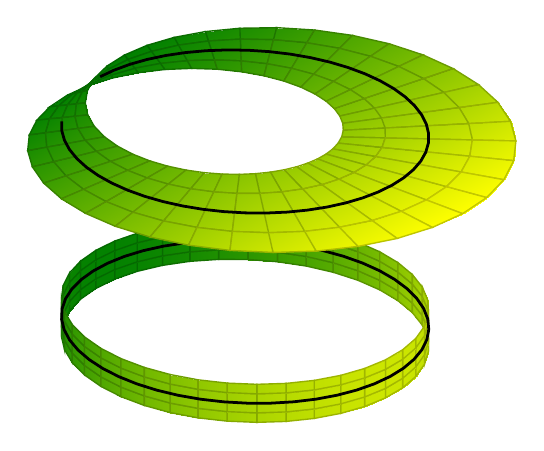
\begin{tikzpicture}[scale=1.25]
\begin{axis}[
    hide axis,
    view={40}{40}
]
\addplot3 [
    surf, shader = faceted interp,
    point meta = x,
    colormap/greenyellow,
    samples = 40,
    samples y = 5,
    z buffer = sort,
    domain = 0:360,
    y domain = -2:2
] (
    {sin(x)},
    {cos(x)},
    {y-20}
  );
  
\addplot3 [
    samples = 50,
    domain = 0:360,
    samples y = 0,
    thick
] (
    {cos(x)},
    {sin(x)},
    {-20}
  );   
  
\addplot3 [
    surf, shader = faceted interp,
    point meta = x,
    colormap/greenyellow,
    samples = 40,
    samples y = 5,
    z buffer = sort,
    domain = 0:360,
    y domain = -1:1
] (
    {(1+0.5*y*cos(x/2)))*cos(x)},
    {(1+0.5*y*cos(x/2)))*sin(x)},
    {0.5*y*sin(x/2)}
  );
  
\addplot3 [
    samples = 50,
    domain = -145:180,
    samples y = 0,
    thick
] (
    {cos(x)},
    {sin(x)},
    {0}
  ); 
\end{axis}
\end{tikzpicture}
\caption{Fiber bundles over a circle} \label{fig:1}
\end{figure}

\section{Example of a fibration}

\begin{ListingEnv}[H]
\begin{lstlisting}
\func neg_neg : \Pi (x : I) -> ((inv seg) @ (inv seg @ x)) = x 
  => \lam x 
    =>  ((\lam x 
      => (\lam i 
        => inv (connAnd (inv seg) i)) (inv seg @ x)) x)
        # (inv ((\lam x 
          => ((\lam x 
            => (\lam i 
              => inv (connAnd seg i)) (seg @ x)) x) # seg) x))
\end{lstlisting}
\end{ListingEnv}

\begin{ListingEnv}[H]
\begin{lstlisting}
\func twist : I = I => Iso=>Path
    \new Iso I I neg neg neg_neg neg_neg
\end{lstlisting}
\end{ListingEnv}

\begin{ListingEnv}[H]
\begin{lstlisting}
\func M : \Pi (x : S1) -> \Type => \lam x => \case x \with {
  | base => I
  | loop i => twist @ i
}
\end{lstlisting}
\end{ListingEnv}

\begin{ListingEnv}[H]
\begin{lstlisting}
\record Moebius (p1 : S1) {
  \field f1 : M(p1)
}
\end{lstlisting}
\end{ListingEnv}

\section{Isomorphism between a fibration and a dependent type}

\begin{ListingEnv}[H]
\begin{lstlisting}
\func family (B : \Type) : \Type => B -> \Type
\end{lstlisting}
\end{ListingEnv}

\begin{ListingEnv}[H]
\begin{lstlisting}
\func total (B : \Type) (F : family B) : \Type 
	=> \Sigma (x : B) (F x)
\end{lstlisting}
\end{ListingEnv}

\begin{ListingEnv}[H]
\begin{lstlisting}
\func trivial (B : \Type) (F : family B) : total B F -> B 
	=> \lam (x : total B F) => x.1
\end{lstlisting}
\end{ListingEnv}

\begin{ListingEnv}[H]
\begin{lstlisting}
\func fiber (A B : \Type) (f : A -> B) (base : B)
   => \Sigma (x : A) (f x = base)
\end{lstlisting}
\end{ListingEnv}

\begin{ListingEnv}[H]
\begin{lstlisting}
\func encode (B : \Type) (F : B -> \Type) (y : B) :
      fiber (total B F) B (trivial B F) y -> F y
   => \lam (x : fiber (total B F) B (trivial B F) y)
   => subst B F x.1.1 y x.2 x.1.2
\end{lstlisting}
\end{ListingEnv}

\begin{ListingEnv}[H]
\begin{lstlisting}
\func decode (B : \Type) (F : B -> \Type) (y : B) :
      F y -> fiber (total B F) B (trivial B F) y
   => \lam (x : F y) => ((y, x), path (\lam i => y))
\end{lstlisting}
\end{ListingEnv}

\begin{ListingEnv}[H]
\begin{lstlisting}
\func decode->encode (B : \Type) (F : family B) (y : B) :
  \Pi (x : F y) -> (encode B F y (decode B F y x)) = x
  => \lam (x : F y)
    => path (\lam i
      => encode
              B
              F
              ((decode B F y x).2 @ i)
              ((y, x), (path (\lam _ => y))))
\end{lstlisting}
\end{ListingEnv}

\begin{ListingEnv}[H]
\begin{lstlisting}
\func encode->decode (B : \Type) (F : family B) (y : B) :
  \Pi (x : fiber (total B F) B (trivial B F) y)
    -> (decode B F y (encode B F y x)) = x
  => \lam (x : fiber (total B F) B (trivial B F) y)
    => path (\lam i
      => (((inv x.2) @ i,
           (pathOverFamily (transport_twist F x.2 x.1.2)) @ i),
          (pathOverFamily ((coe_path (inv x.2) rfl rfl)
                      # (comp-assoc (inv (inv x.2)) rfl rfl)
                         # (refl-right ((inv (inv x.2)) # rfl))
                            # (refl-right (inv (inv x.2)))
                               # (inv_inv x.2))) @ i))
          \where
            \func transport_twist {A : \Type} (B : A -> \Type)
                                  {a b : A}
                                  (p : a = b) (x : B a) :
              transport B (inv p) (transport B p x) = x
              => J (\lam z (p' : a = z)
                => transport B (inv p') (transport B p' x) = x) rfl p
\end{lstlisting}
\end{ListingEnv}

\begin{ListingEnv}[H]
\begin{lstlisting}
\func hFiber=DependentTypeParameterized (B : \Type) 
	(F : family B) (y : B) : 
	(fiber (total B F) B (trivial B F) y) = (F y)
  => Iso=>Path 
  	(\new Iso 
  		(fiber (total B F) B (trivial B F) y) 
  		(F y) 
  		(encode B F y) 
  		(decode B F y) 
  		(encode->decode B F y) 
  		(decode->encode B F y))
\end{lstlisting}
\end{ListingEnv}

\begin{ListingEnv}[H]
\begin{lstlisting}
\func Fibration=DependentType (B : \Type) (F : family B) : 
  (fiber (total B F) B (trivial B F)) = F
  => path (\lam i y
    => (hFiber=DependentTypeParameterized B F y) @ i)
\end{lstlisting}
\end{ListingEnv}

\Conc

\begin{otherlanguage}{english}
\printbibliography[%{}
    heading=bibintoc%
    ,title=Bibliography
]
\end{otherlanguage}

\end{document}
